As our differentiable basis set framework lets us differentiate through the whole basis set fitting procedere, we can choose to replace the constant basis functions that are commonly used in DFT calculation with adaptive ones which can adopt to the local chemical environment. First approaches in this direction were done by .... and recently with the rise of machine learing approches Linear fitted coefficient (...) and by a gaussian process predicted coefficients have been tried out. Adaptive exponents inside the Gaussian basis functions have been avoided so far as they require to differentiate through the integrals. But now owr framework allows us to to learn the coefficients and exponents used in dft calculations jointly. We mainly restrict our analysis to minimal basis sets, specificly the STO-3G and the STO-6G\cite{STO-3G} minimal basis sets, as they are exspected to profit the most from these improvements. We then use a small graph neural network, as described in \ref{Machine learning} to predict the exponents and coefficients of these Basis sets.
\section{Multi Step Pretraining}
As the differential basis functions are currently very slow and use a lot of vram compared to what is common in machine learing we cannot reach a very high number of iterations in learning. To compensate for this we using multiple pretraing procedere to improve the speed at which the neural network is learing. At first we let the network predict predict atomwise features, which don't require a evaluation of the differentiable integrals and can therefor be evaluated very quickly.
\subsection{Pretraining on atomwise properties}
We first evaluate the Neural network on atomwise properties to let it produce a kind of "physical intuition" before letting it work on the hard task of reliable predicting cefficients and expoenents for each atoms. For the features we borrow from the labels that have been produced for the orbital free model.
We predict the features by adding an extra linear output head at the last layer of the neural network. 
The following feature were predicted:
\begin{enumerate}
    \item Atomic number of each atom, $Z_i$.
    \item Coulomb potential from each neighboring atom, $-\sum\limits_{a \in \mathcal{N}(i)} \frac{Z_a}{|e_{i-a}|}$.
    \item Sum of Coulomb forces acting on the current atom, $\sum\limits_{a \in \mathcal{N}(i)} \frac{Z_a Z_i}{|e_{i-a}|^2}$.
    \item Effective number of electrons, $\sum\limits_{\mu} \text{mask}(i)_\mu p_\mu w_\mu$.
    \item Effective charge: Atomic number minus the effective number of electrons.
    \item Integrated kinetic gradient.
    \item Integrated external energy of this atom.
    \item Integrated Hartree gradient.
    \item Integrated exchange-correlation (xc) gradient.
    \item Integrated total energy gradient.
\end{enumerate}
where $\text{mask(i)}_\mu =
\begin{cases}
1, & \text{if } \omega_\mu(\mathbf{r}) \text{ is centered on } \mathbf{R_i} \\
0, & \text{else}
\end{cases}$

\subsection{Orbitals Deltalearing to bigger basis set}
For the main traing step we train the basis set by fitting the orbitals produced by the largely bigger basis set 6-31G(2df,p) with the smaller adaptive basis set.
We define our loss as the sum of the L2 norms between the orbitals produced by the bigger basis set and the orbitals which of the smaller basis set which we fit to the bigger basis set using density fitting. As orbitals should be orthonormal to each other we also enforce this property during density fitting. The loss function is defined as
\begin{align}
    \text{Loss}(\Phi') = \underset{\{\phi_i\}_{i=1,...,N_e} \text{pairwise orthonormal}}{\text{min}}\sum\limits_{i=1}^{N_e} \int (\phi_i(\mathbf{r})-\phi'_i(\mathbf{r}))^2 d\mathbf{r}.
\end{align}
Where $\Phi' = \{\phi'_i\}_{i=1,...,N_e}$ are the occupied orbitals produced by the bigger basis set and $\Phi = \{\phi_i\}_{i=1,...,N_e}$ are the orbitals defined on the basis functions of our smaller basis  which are fiited to the bigger basis set. The solution of this equation in components leads us to equation \eqref{adaptive_loss_final}.
The derivation of this equation can be found in appendix \ref{derivation_adaptive_loss}, it is identical to the common precedure of data whitening applied to the original orbitals.
\begin{align}\label{adaptive_loss_final}
    \text{Loss} &= \sum_i C_{i,\mu} \langle\eta_\mu|\eta_\nu\rangle C_{i,\nu} - 2 C_{i,\mu} \langle\eta_\mu|\tilde\eta_\nu\rangle \tilde C_{i,\nu} + \tilde C_{i,\mu} \langle\tilde \eta_\mu|\tilde \eta_\nu\rangle \tilde C_{i,\nu}\\
     C_{i,\mu}&= \sum_{j} A^{-\frac{1}{2}}_{i,j} \langle\eta_\mu|\eta_\nu\rangle^{-1}_{\mu,\nu} \langle\eta_\nu|\tilde\eta_\gamma\rangle \tilde C_{j,\gamma}\\
    A_{i,j}&=\tilde C_{i,\sigma}\langle\tilde \eta_\sigma|\eta_\mu\rangle \langle\eta_\mu|\eta_\nu\rangle^{-1}_{\mu,\nu} \langle\eta_\nu|\tilde\eta_\gamma\rangle \tilde C_{i,\gamma}\\
\end{align}
As we now have a formulation for the loss in terms of simple basis integrals we can then insert the dependency of the integrals on the contractions coefficients $\mathbf{A}$ and exponents $\mathbf{\alpha}$ and their respective dependency on the parameters of the neural network, which we will denote as $\Omega$, as well as the molecule geometry $\mathcal{M}$. Affected are the symmetric overlap metricies $\langle\eta(\alpha[\mathcal{M},\Omega],A[\mathcal{M},\Omega])_\mu|\eta(\alpha[\mathcal{M},\Omega],A[\mathcal{M},\Omega])_\nu\rangle$ and the asymmetric overlap metricies $\langle\eta(\alpha[\mathcal{M},\Omega],A[\mathcal{M},\Omega])_\mu|\tilde\eta_\nu\rangle$. The overlap metricies of the target basis $\langle\tilde \eta_\mu|\tilde \eta_\nu\rangle$ have no further dependencies and can therefor be omitted from the loss. From here on out we can train the model, as we did in the privous section, using stochastic gradient decent on the dataset QM9 to minimize the loss function.
\subsection{Gradient decent on total energy}
Training the model to provide basis functions which can produce densities which are closer to these of the bigger basis set is a good start, as, in theory, it lets kohn sham generate better orbitals and therefor also better energies. But as our adaptive basis set is much smaller then the one we are using as reverence, there is a limit to how well the orbitals can be fitted. Even worse trying to fit the densities to closely could lead to unphysical basis functions which produce better fits but worse energies. If we want to optimize our predicted basis sets to produce better energies we should optimize the total energy direcly. As we want to predict the ground state energy of a molecule, which means the state with the lowest energy, we want to find predict the basis set which produces the lowest energy. We therefor can use the total energy as a loss function. The total energy in kohn sham is defined as
\begin{align}
    E_{\text{tot}}[\Phi] = T_S[\Phi] + V_{\text{ext}}[\Phi] + V_{\text{H}}[\Phi] + V_{\text{xc}}[\Phi] + E_{\text{NN}}
\end{align}
Our differentiable integrals let us compute each of these functionals in a differentiable way and insert our dependencies on the contraction coefficients, the exponents and at last the parameters of the neural network, but we also need to keep in mind that the orbitals calculated by kohn sham $\Phi = \{\phi_i\}_{i=1,...,N_e}$ are also dependent on these parameters. Let us now insert these dependencies and perform the derivative towards the model parameters:

\begin{align}
    E_{\text{tot}}[\Phi(\alpha[\mathcal{M},\Omega],&A[\mathcal{M},\Omega]),\alpha[\mathcal{M},\Omega],A[\mathcal{M},\Omega]] \\
    &= T_S[\Phi(\alpha[\mathcal{M},\Omega],A[\mathcal{M},\Omega]),\alpha[\mathcal{M},\Omega],A[\mathcal{M},\Omega]] \nonumber\\
    &+ V_{\text{ext}}[\Phi(\alpha[\mathcal{M},\Omega],A[\mathcal{M},\Omega]),\alpha[\mathcal{M},\Omega],A[\mathcal{M},\Omega]] \nonumber\\
    &+ V_{\text{H}}[\Phi(\alpha[\mathcal{M},\Omega],A[\mathcal{M},\Omega]),\alpha[\mathcal{M},\Omega],A[\mathcal{M},\Omega]] \nonumber\\
    &+ V_{\text{xc}}[\Phi(\alpha[\mathcal{M},\Omega],A[\mathcal{M},\Omega]),\alpha[\mathcal{M},\Omega],A[\mathcal{M},\Omega]] + E_{\text{NN}}\nonumber\\
        \frac{\partial E_{\text{tot}}[...]}{\partial \Omega}
    &= \frac{\partial E_{\text{tot}}[...]}{\partial \phi_i[...]}\frac{\partial \phi_i[...]}{\partial \Omega} + \frac{\partial E_{\text{tot}}[...]}{\partial \alpha[...]}\frac{\partial \alpha[...]}{\partial \Omega} + \frac{\partial E_{\text{tot}}[...]}{\partial A[...]}\frac{\partial A[...]}{\partial \Omega}
\end{align}
If we now choose the orbitals to be ground state orbitals, of the current basis set, then by definition the derivative of the total energy with respect to the orbitals is zero  $\frac{\partial E_{\text{tot}}[...]}{\partial \phi_i[...]}=0$. This means that we can remove the dependency of the orbitals on the model paramters and can still calculate the gradient of the total energy with respect to the model parameters. We therefor propose the following training scheme: First we calculate use the current model to predict the basis for our current molecule. Then we fix this basis and use pyscf's\cite{pyscf} implementation of kohn sham to compute the ground state orbitals in a non differantiable way. Then we take these orbitals and, using our differatiable integrals framework, calculate the total energy of the molecule with enabled autograd. We can than use the calculated total energy as our loss function for which we can calculate the gradient with respect to the model parameters. Then we can use gradient decent to update the parameters of the model. This way we can apply stochastic gradient decent to minimize the total energies of the molecules in the QM9 dataset. The major drawback of this approach is that it needs a complete kohm sham calculation in each steps and the calculation of the total energy using the differentiable integrals is also very slow and needs a lot of ram. To lower the load a bit we used density fitting using the hartree fitting method with an even tempered 3.0 basis set build on our minimal basis set to emulate the calculation of the hartree energy $E_$. Even with these improvements we could only run a single calculation on a gpu at a time while also strongly utilicing the cpu. We therefor could only run a few iterations of this training scheme.
\Section{Evaluation}
To evaluate our adaptive basis sets we choose 210 molecules evenly distributed over QM9 and run full spin restricted kohn sham calculations to obtain ground state densities and energies for these basis sets.

\begin{figure}
    \centering
    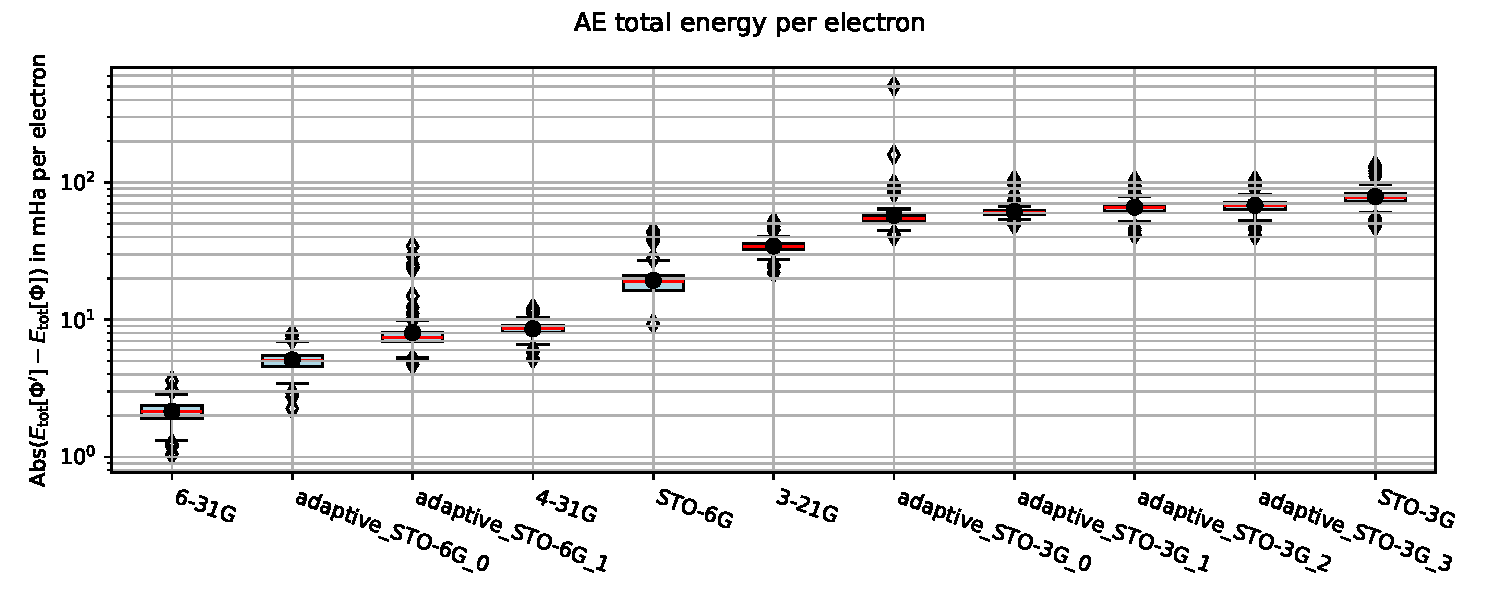
\includegraphics[width=0.75\textwidth]{chapters/results/results_images/adaptive_basis_functions/total_energy_adaptive_basis_sets}
    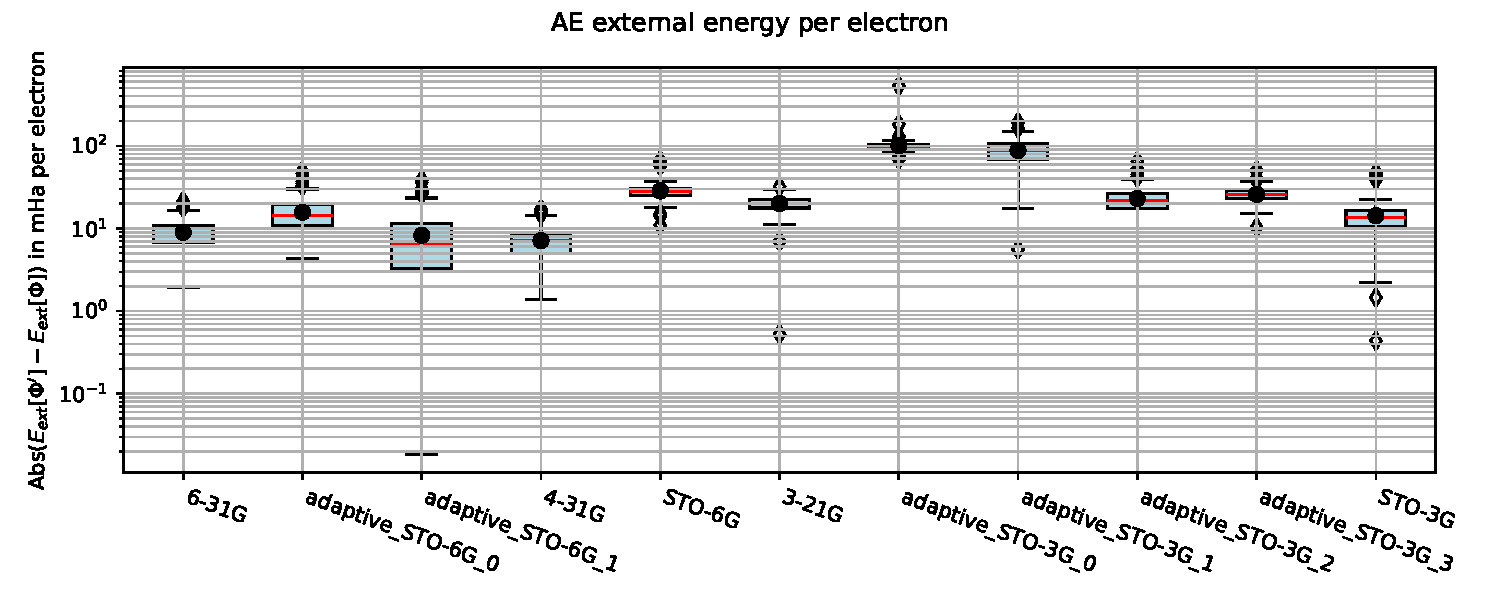
\includegraphics[width=0.75\textwidth]{chapters/results/results_images/adaptive_basis_functions/coulomb_energy_adaptive_basis_sets}
    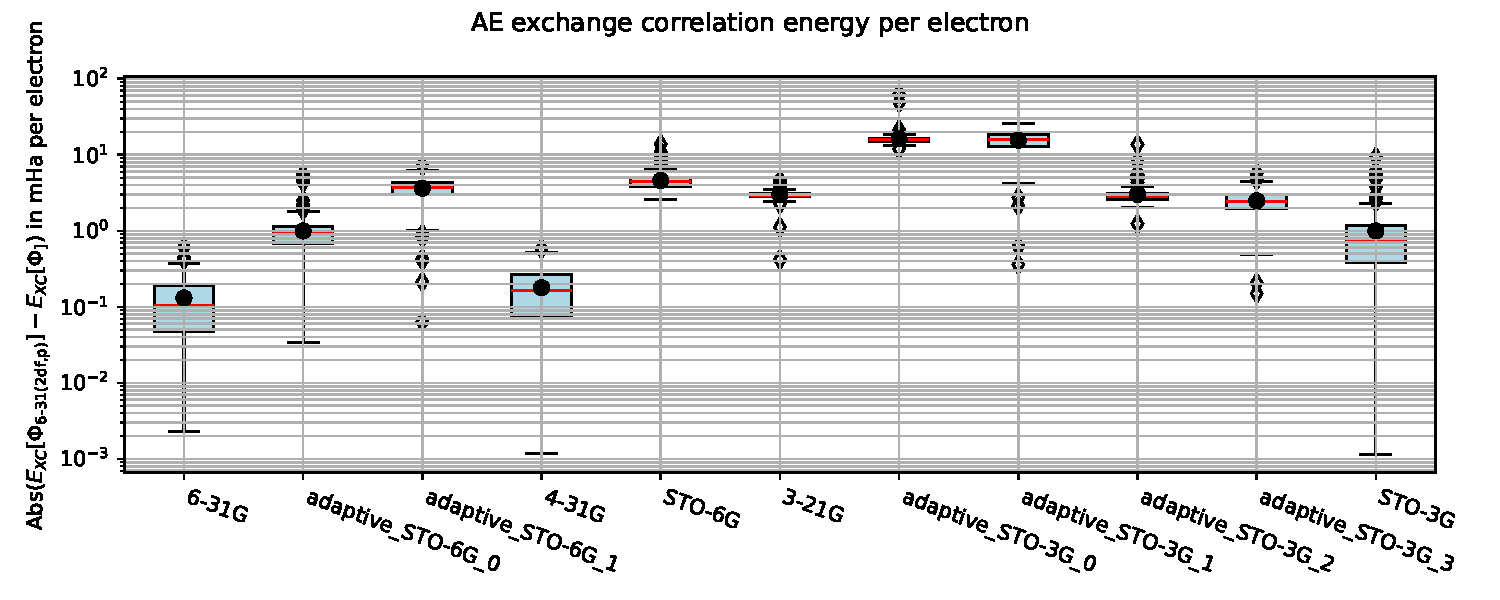
\includegraphics[width=0.75\textwidth]{chapters/results/results_images/adaptive_basis_functions/exchange_correlation_energy_adaptive_basis_sets}
    \caption{Boxplots(\ref{boxplots}) of the AE for the different energies produced by kohn sham on the different classical and adaptive basis functions on 210 Molecules evenly distributed over QM9, compared to calculations on the basis set "6-31G(2df,p)".} \label{fig:AE_energies_adaptive_basis_sets}
\end{figure}




\begin{figure}
    \centering
    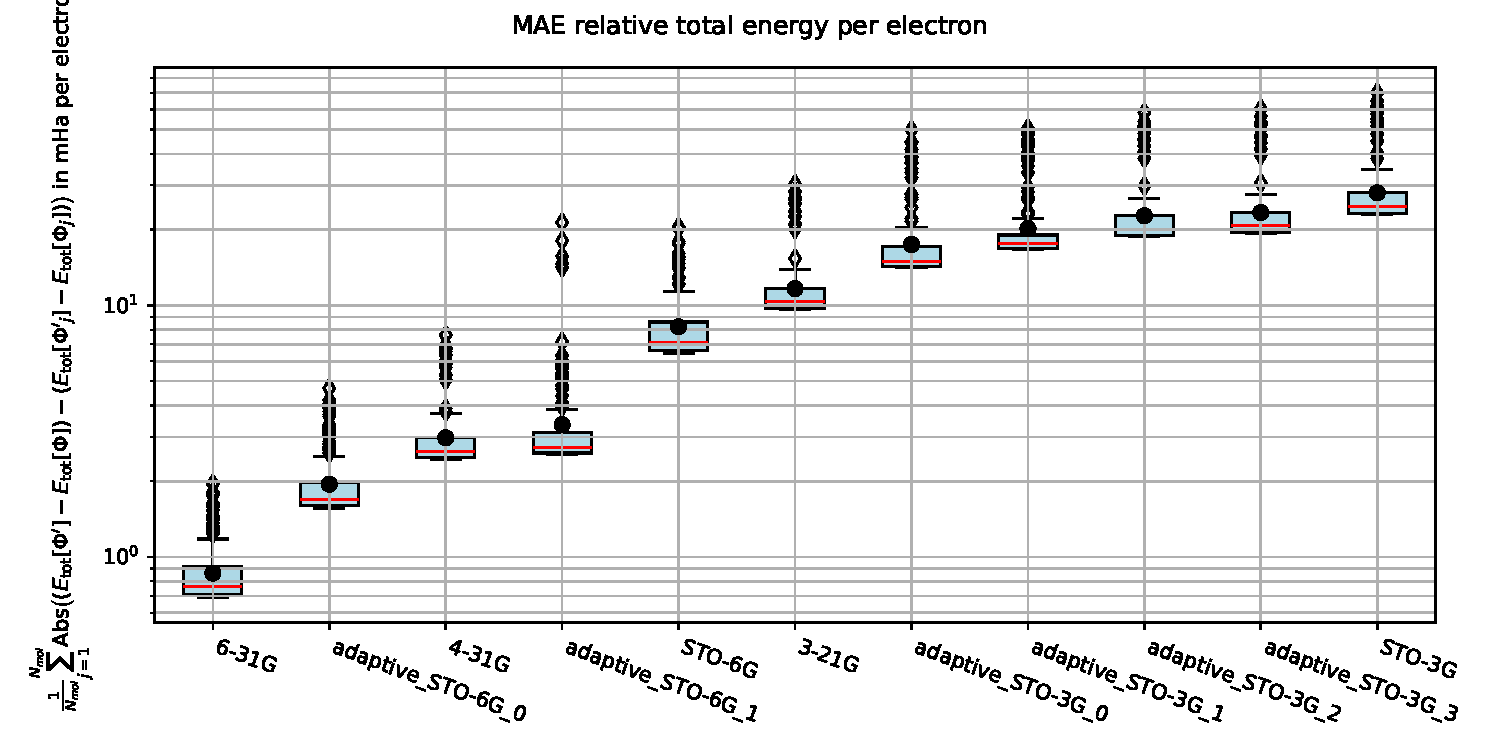
\includegraphics[width=0.75\textwidth]{chapters/results/results_images/adaptive_basis_functions/relative_total_energy_adaptive_basis_sets}
    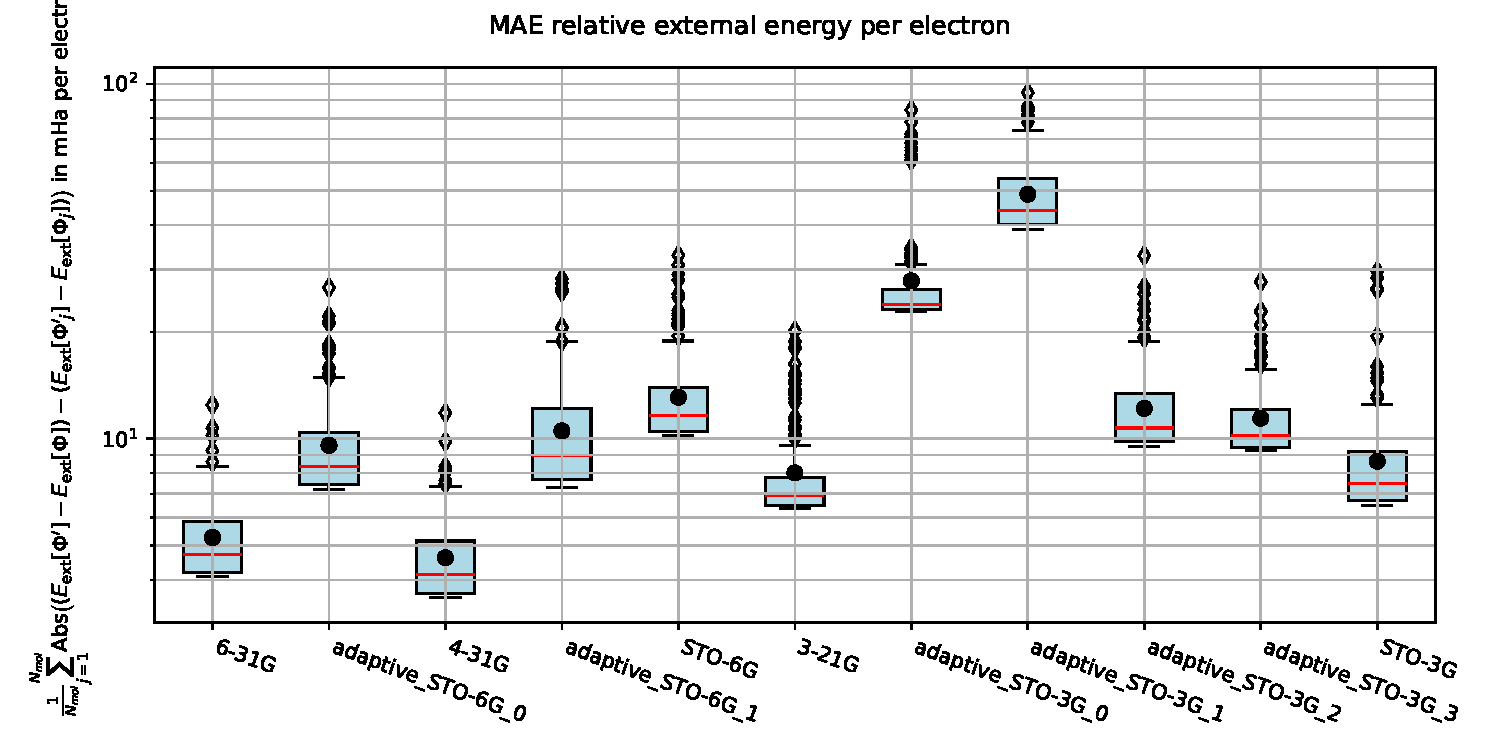
\includegraphics[width=0.75\textwidth]{chapters/results/results_images/adaptive_basis_functions/relative_coulomb_energy_adaptive_basis_sets}
    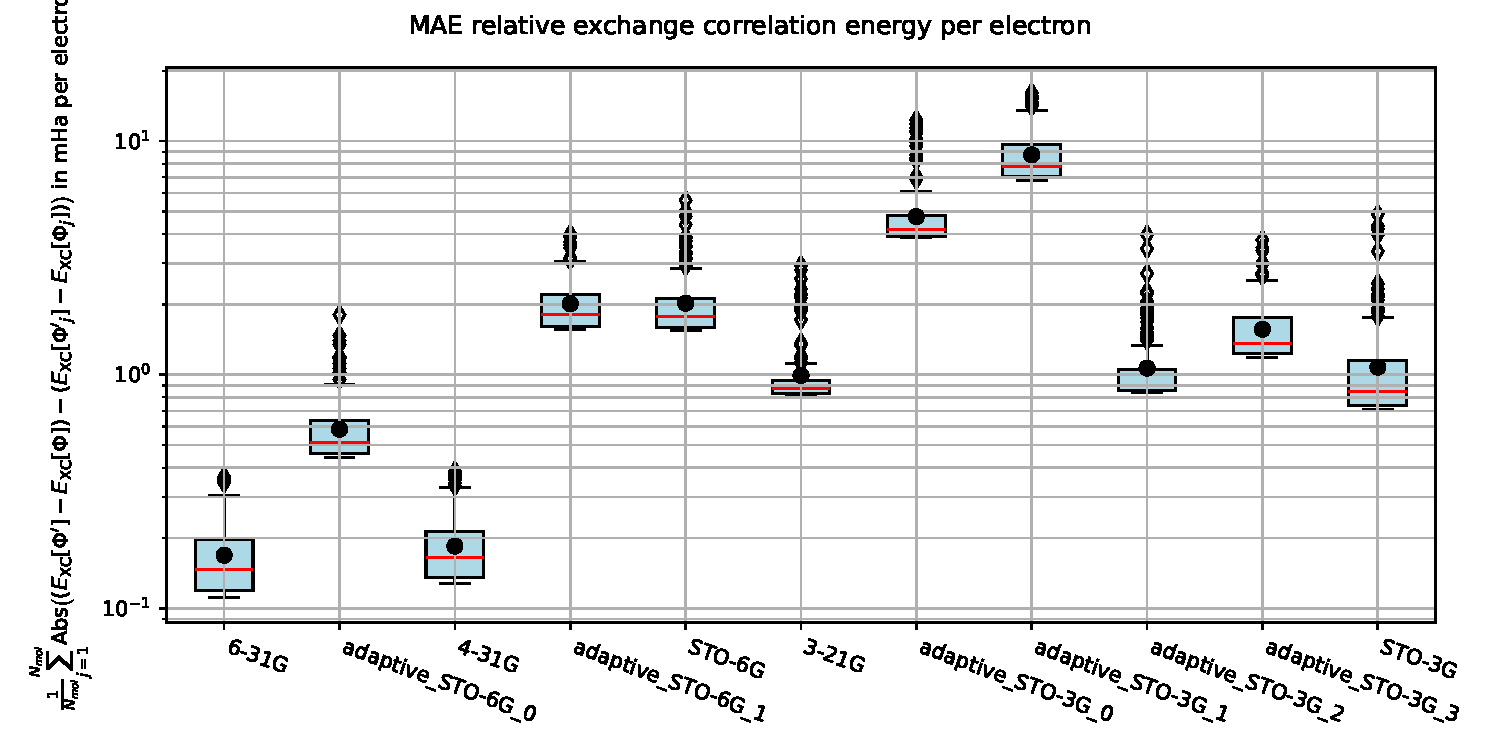
\includegraphics[width=0.75\textwidth]{chapters/results/results_images/adaptive_basis_functions/relative_exchange_correlation_energy_adaptive_basis_sets}
    \caption{Boxplots(\ref{boxplots}) of the AE for the relative energies errors(\ref{relative_energy_errors}) produced by kohn sham on the different classical and adaptive basis functions on 210 Molecules evenly distributed over QM9, compared to calculations on the basis set "6-31G(2df,p)".}
    \label{fig:AE_relative_energies_adaptive_basis_sets}
\end{figure}

\begin{figure}
    \centering
    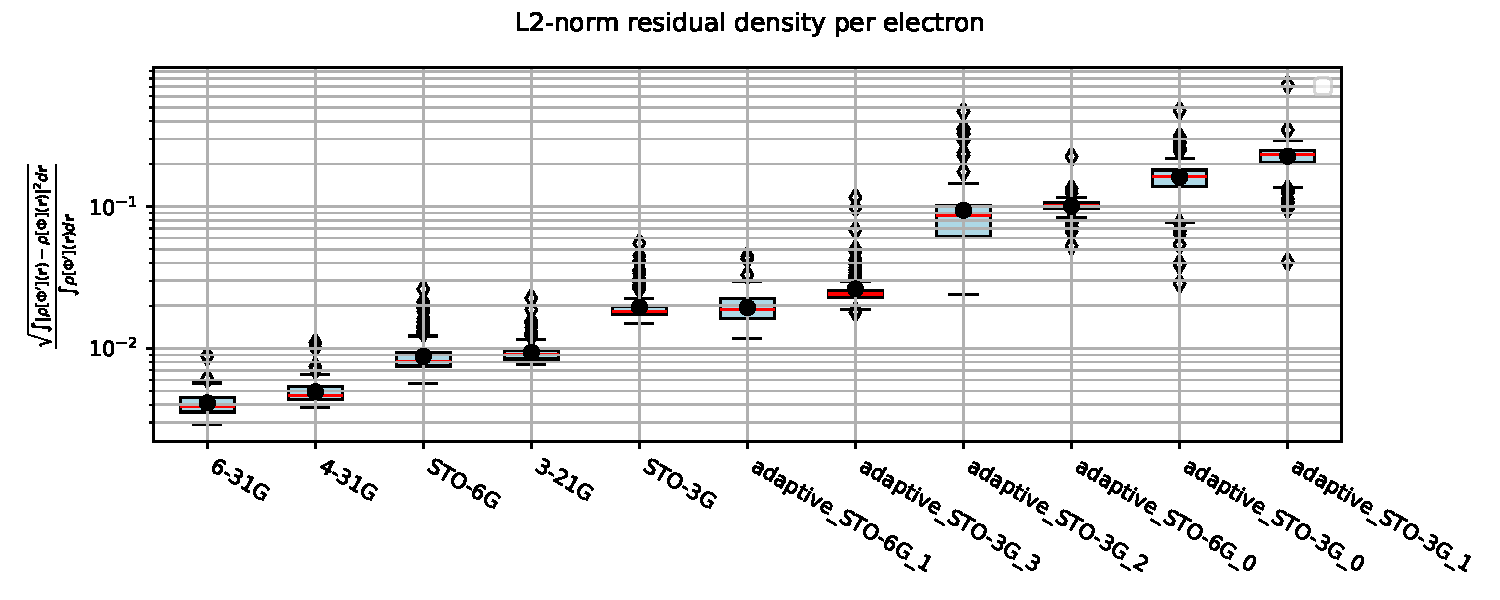
\includegraphics[width=0.75\textwidth]{chapters/results/results_images/adaptive_basis_functions/L2-norm_residual_density_per_electron_adaptive_basis_sets}
    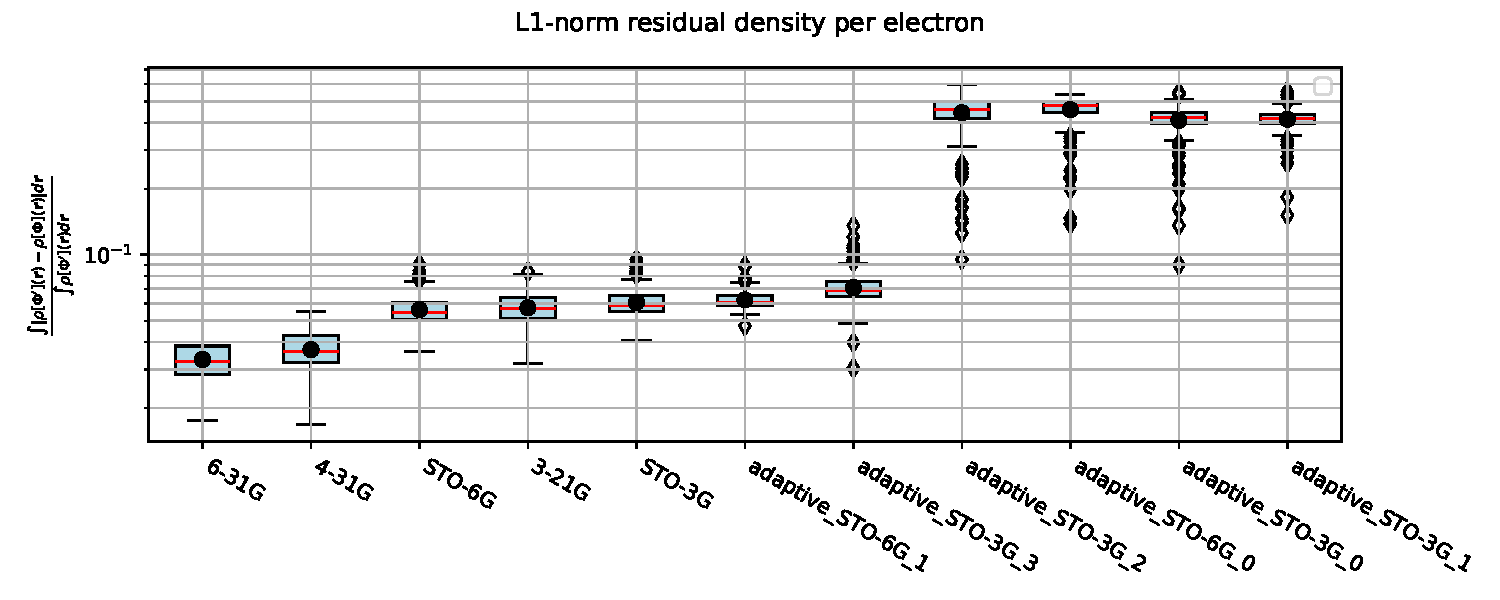
\includegraphics[width=0.75\textwidth]{chapters/results/results_images/adaptive_basis_functions/L1-norm_residual_density_per_electron_adaptive_basis_sets}
    \caption{Boxplots(\ref{boxplots}) of the difference in densities produced by kohn sham on the different classical and adaptive basis functions on 210 Molecules evenly distributed over QM9, compared to calculations on the basis set "6-31G(2df,p)".}
    \label{fig:residual_density_adaptive_basis_sets}
\end{figure}

\begin{figure}
    \centering
    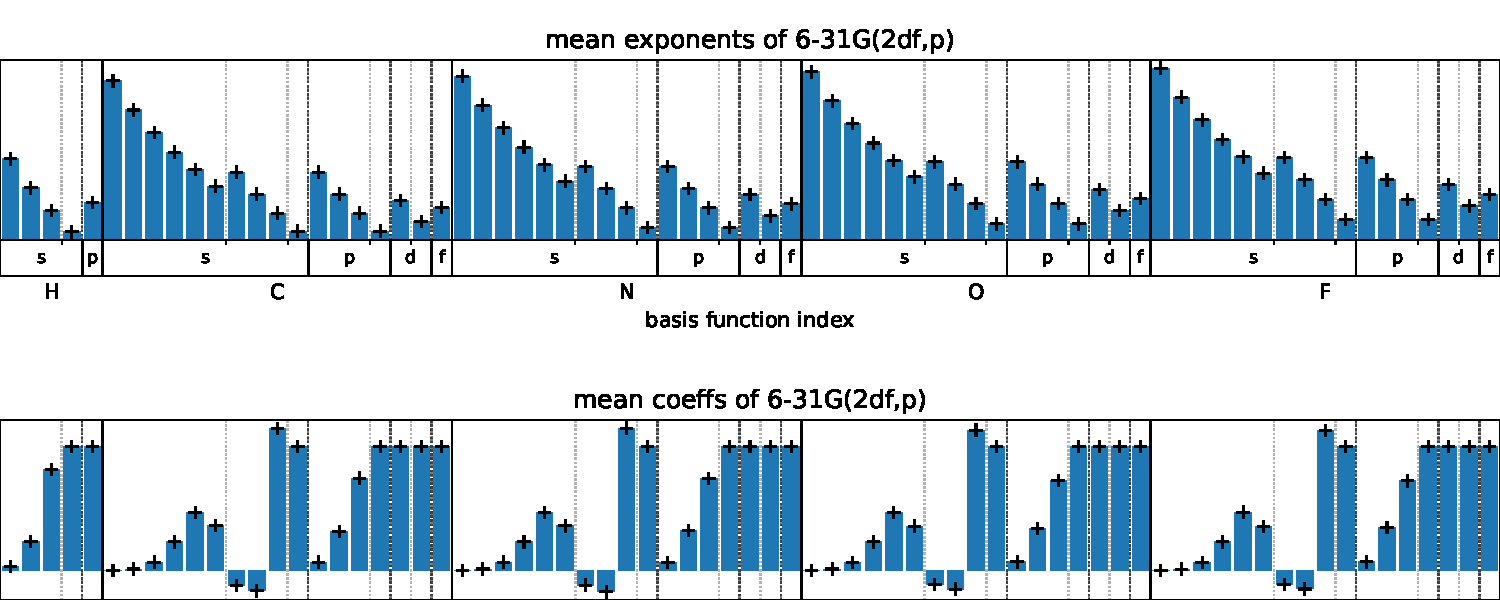
\includegraphics[width=0.75\textwidth]{chapters/results/results_images/adaptive_basis_functions/mean_exps_and_coeffs6-31G(2df,p)}
    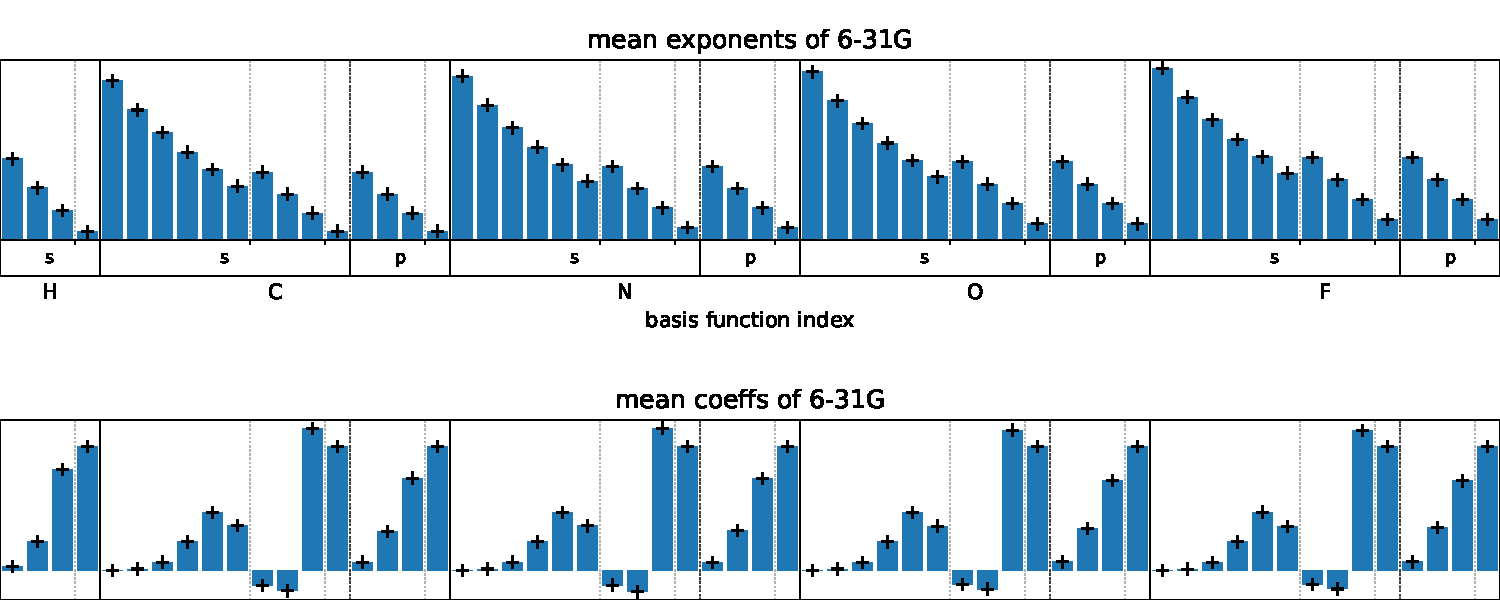
\includegraphics[width=0.75\textwidth]{chapters/results/results_images/adaptive_basis_functions/mean_exps_and_coeffs6-31G}
    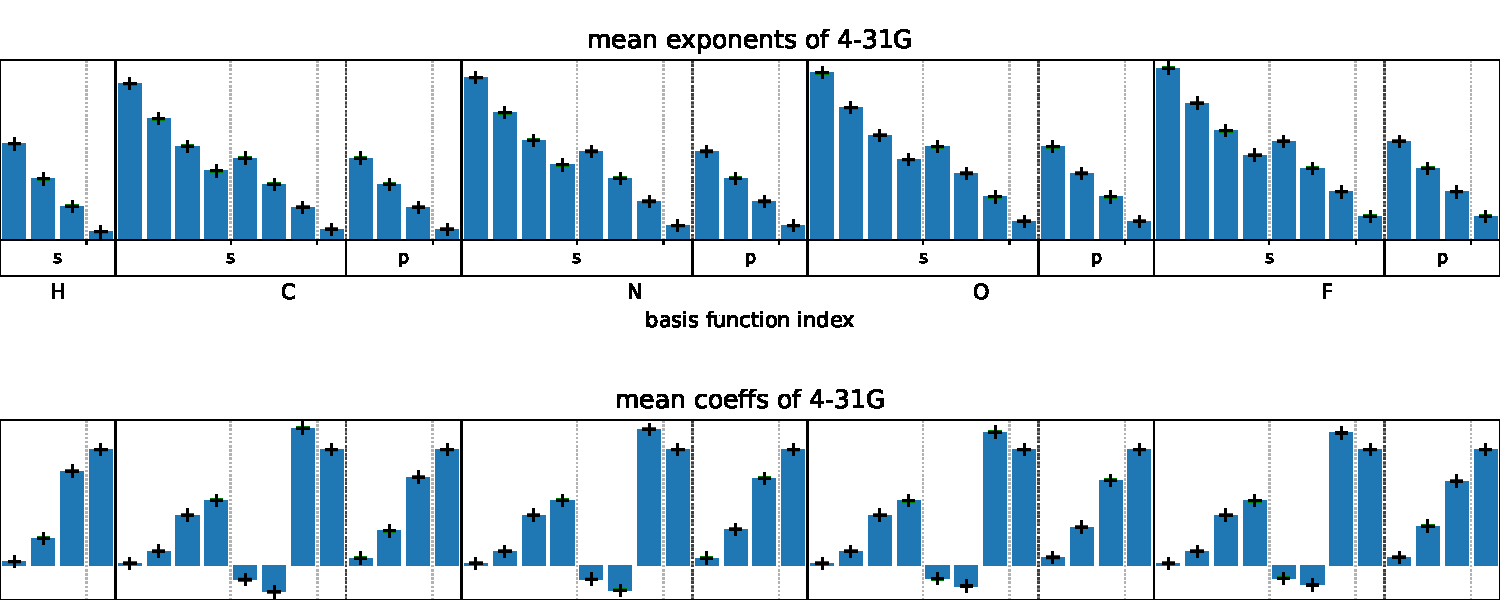
\includegraphics[width=0.75\textwidth]{chapters/results/results_images/adaptive_basis_functions/mean_exps_and_coeffs4-31G}
    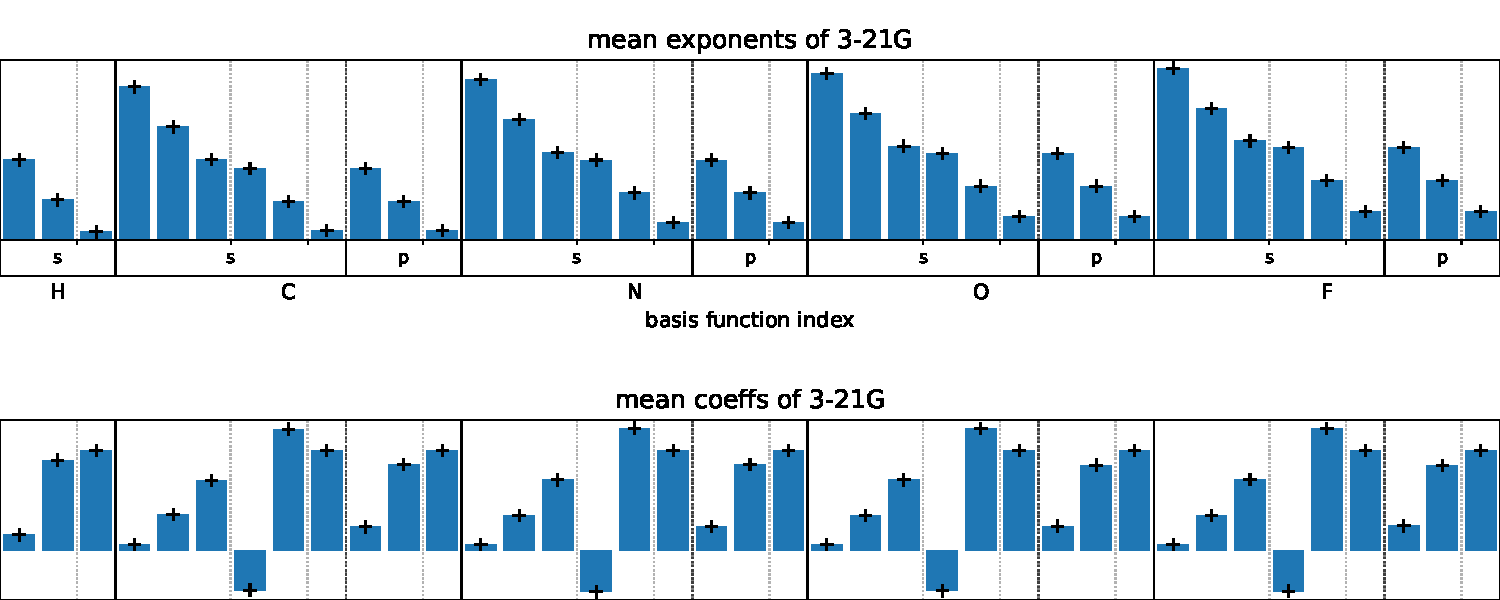
\includegraphics[width=0.75\textwidth]{chapters/results/results_images/adaptive_basis_functions/mean_exps_and_coeffs3-21G}
    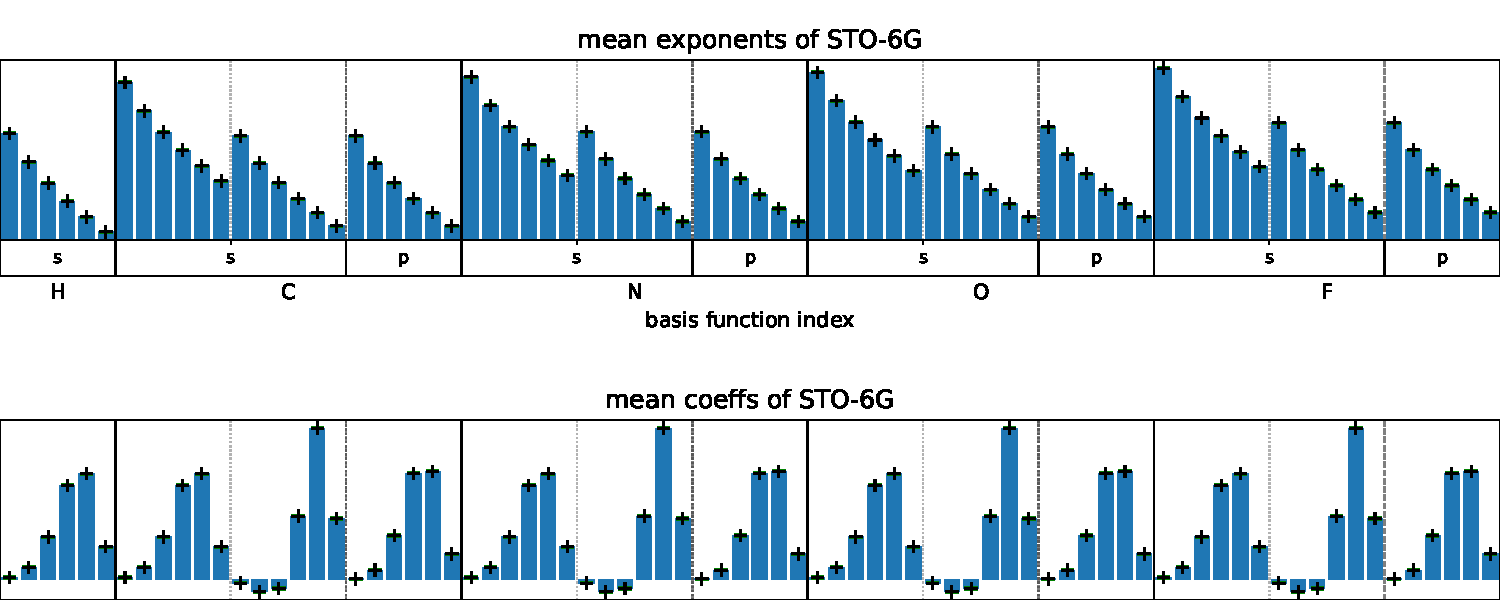
\includegraphics[width=0.75\textwidth]{chapters/results/results_images/adaptive_basis_functions/mean_exps_and_coeffsSTO-6G}
    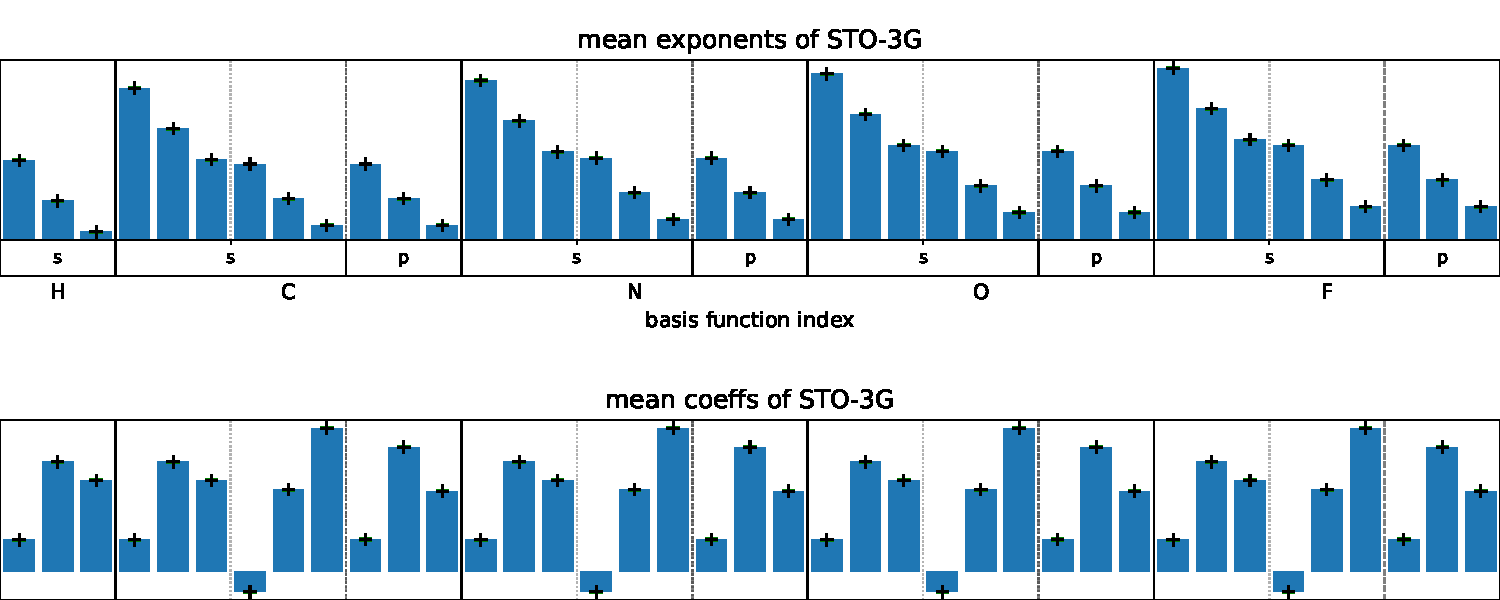
\includegraphics[width=0.75\textwidth]{chapters/results/results_images/adaptive_basis_functions/mean_exps_and_coeffsSTO-3G}
\end{figure}

\begin{figure}
    \centering
    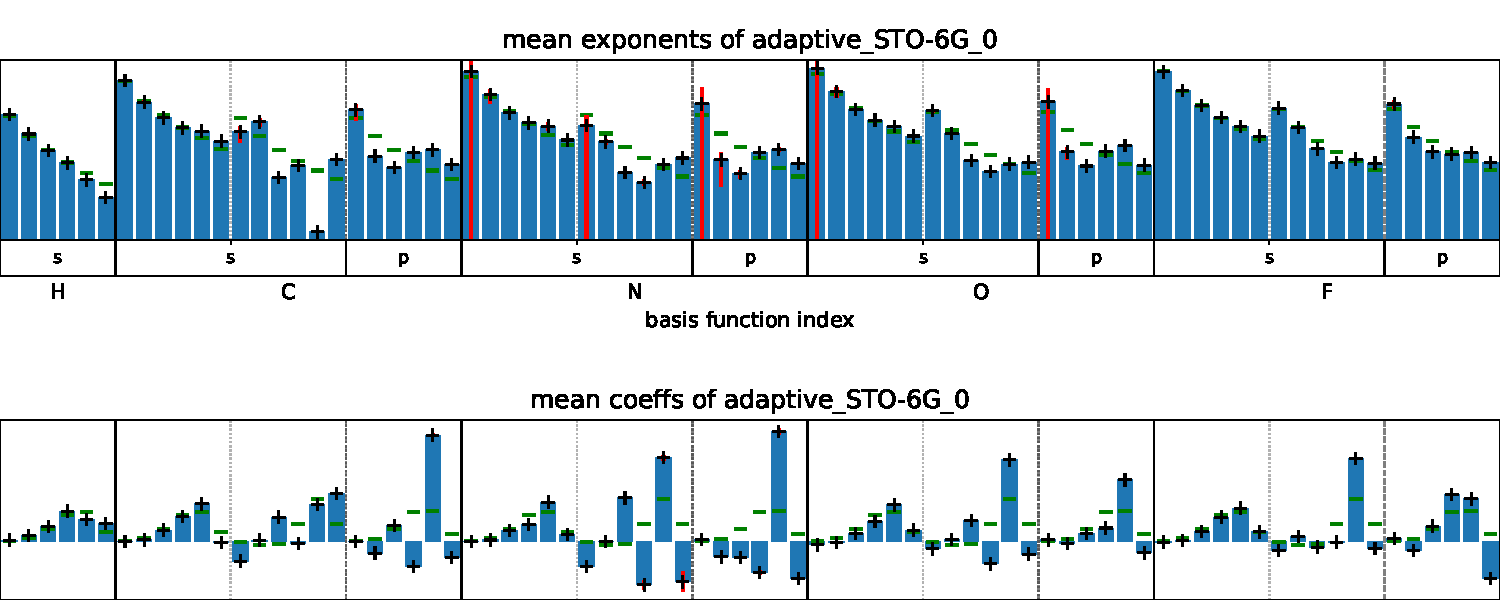
\includegraphics[width=0.75\textwidth]{chapters/results/results_images/adaptive_basis_functions/mean_exps_and_coeffsadaptive_STO-6G_0}
    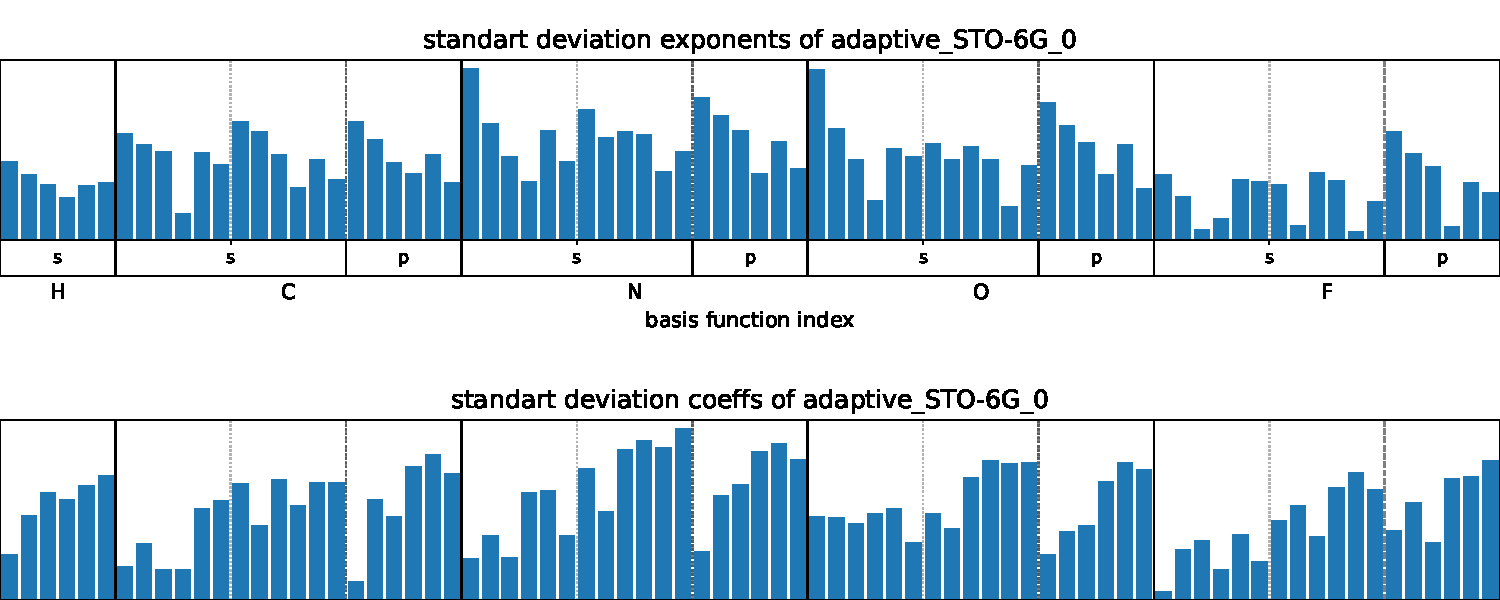
\includegraphics[width=0.75\textwidth]{chapters/results/results_images/adaptive_basis_functions/std_exps_and_coeffsadaptive_STO-6G_0}
    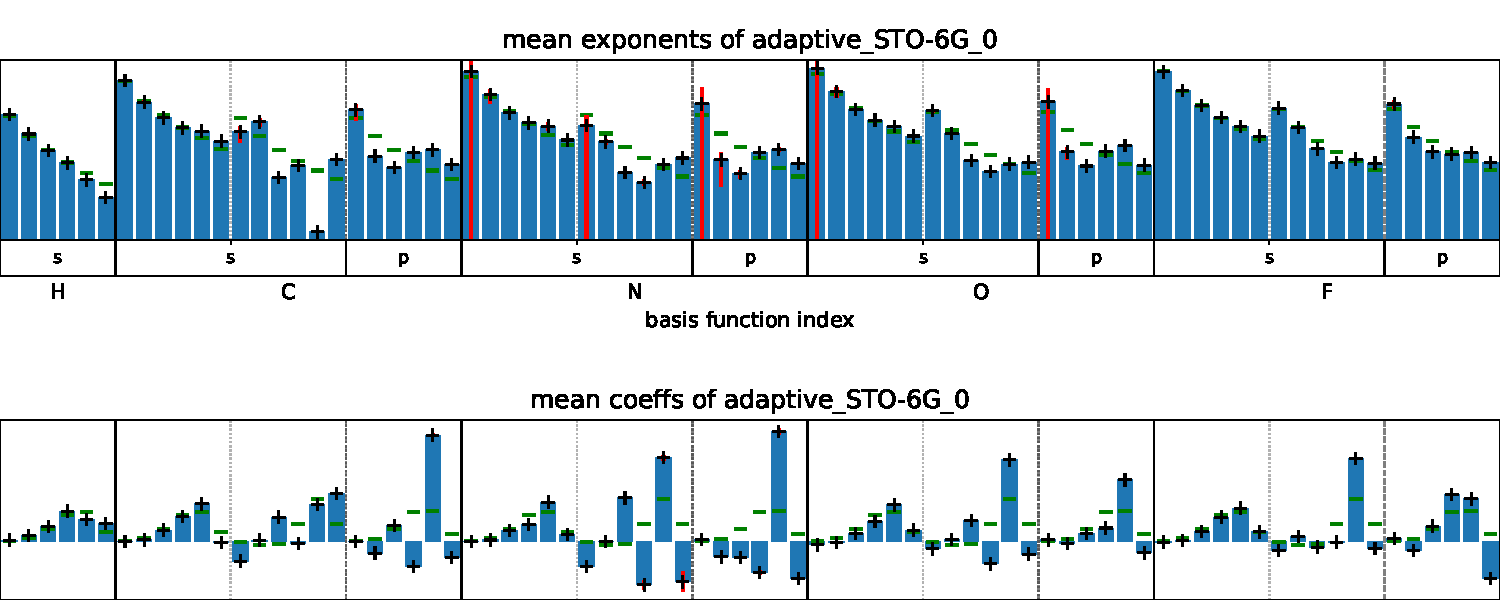
\includegraphics[width=0.75\textwidth]{chapters/results/results_images/adaptive_basis_functions/mean_exps_and_coeffsadaptive_STO-6G_0}
    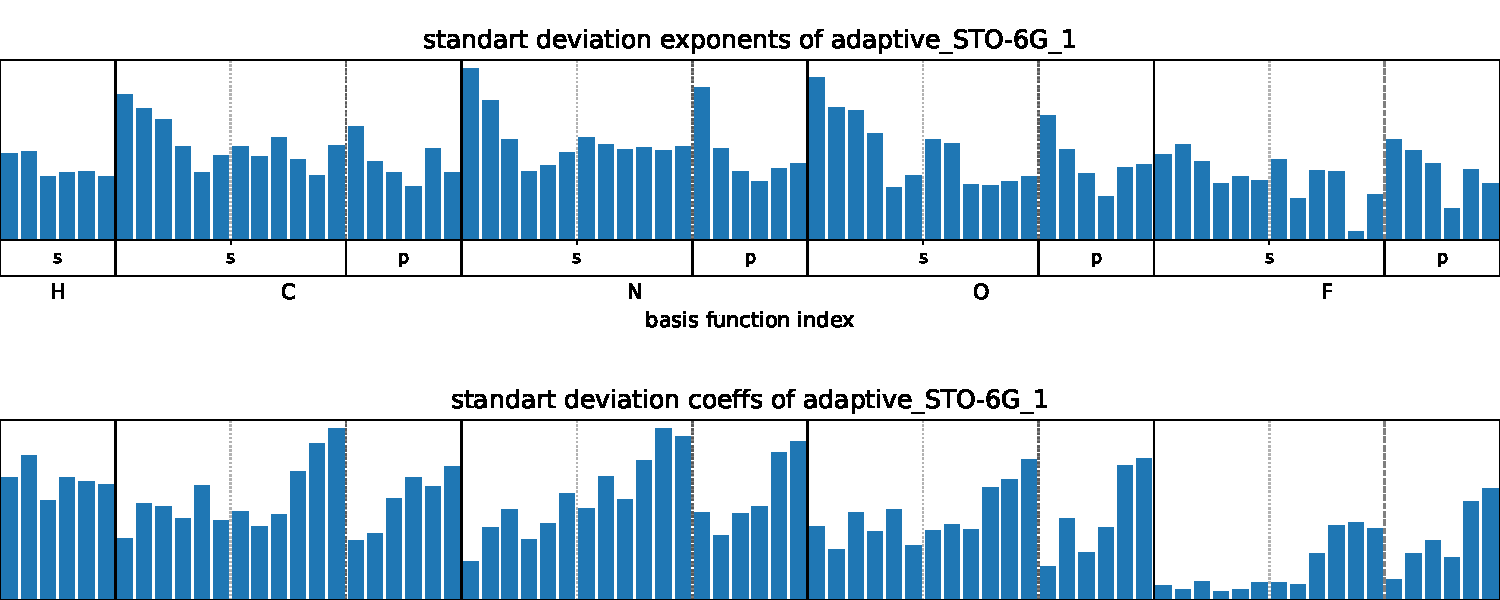
\includegraphics[width=0.75\textwidth]{chapters/results/results_images/adaptive_basis_functions/std_exps_and_coeffsadaptive_STO-6G_1}
\end{figure}

\begin{figure}
    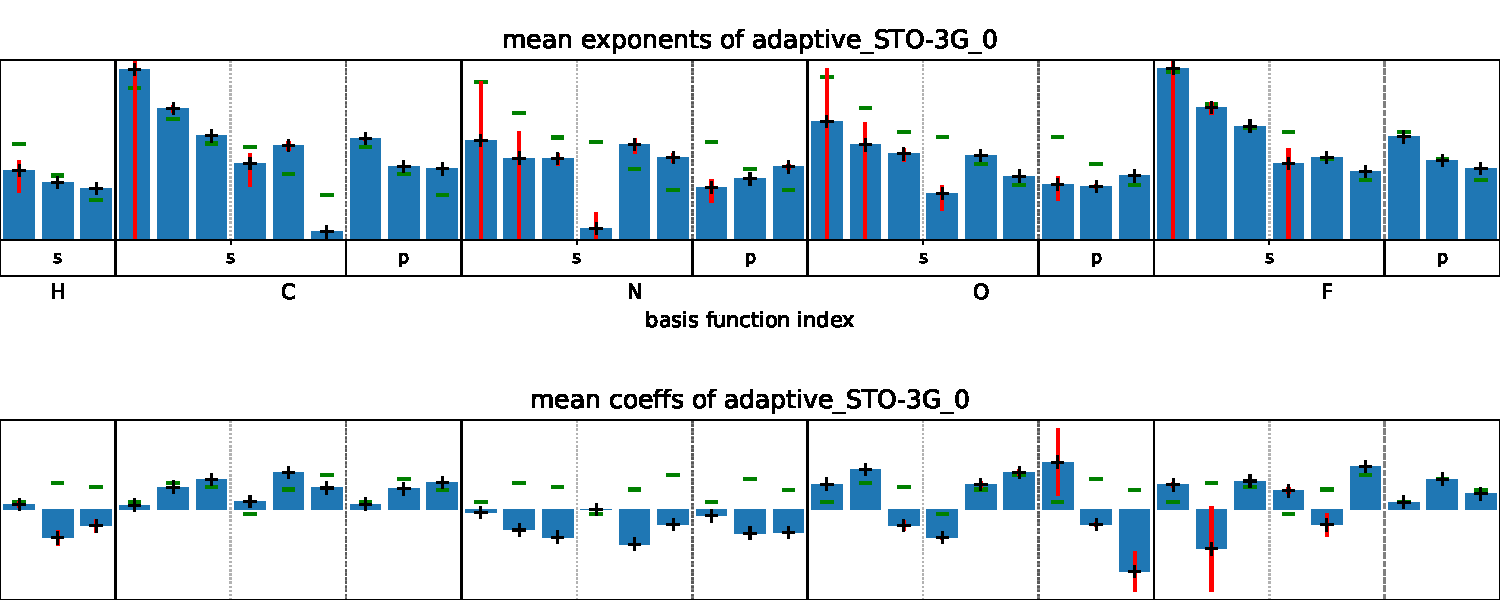
\includegraphics[width=0.75\textwidth]{chapters/results/results_images/adaptive_basis_functions/mean_exps_and_coeffsadaptive_STO-3G_0}
    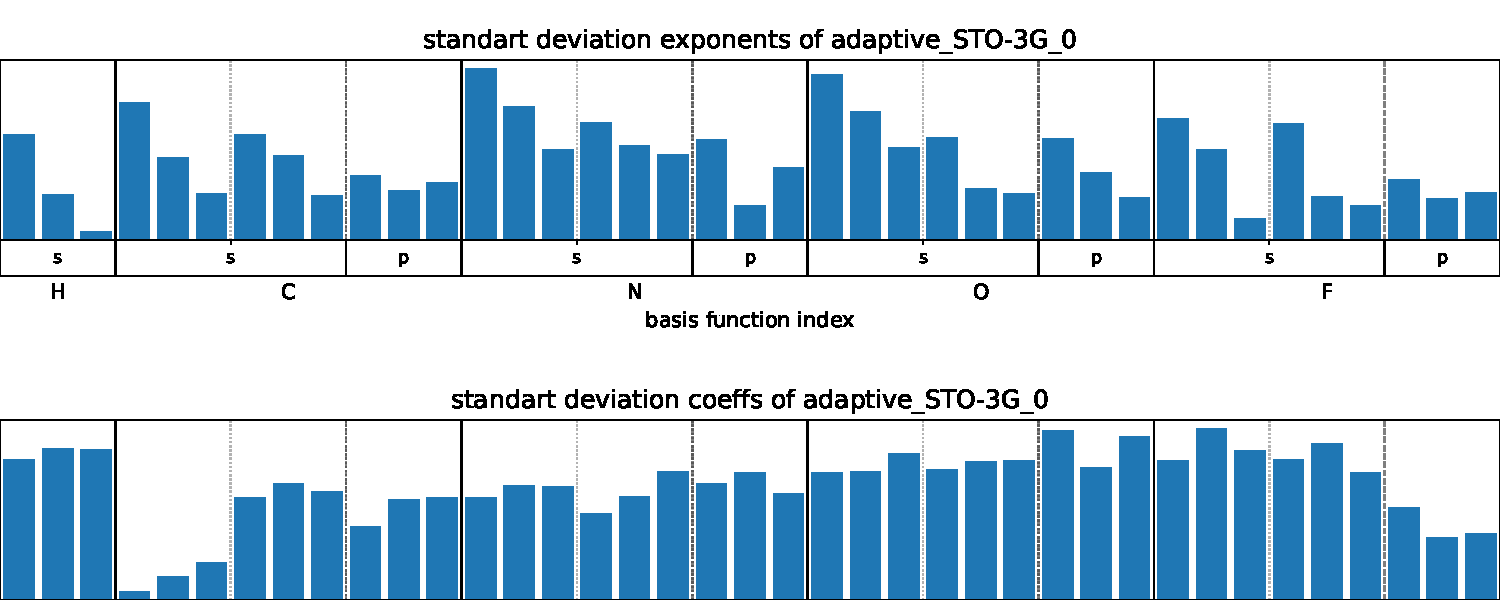
\includegraphics[width=0.75\textwidth]{chapters/results/results_images/adaptive_basis_functions/std_exps_and_coeffsadaptive_STO-3G_0}
    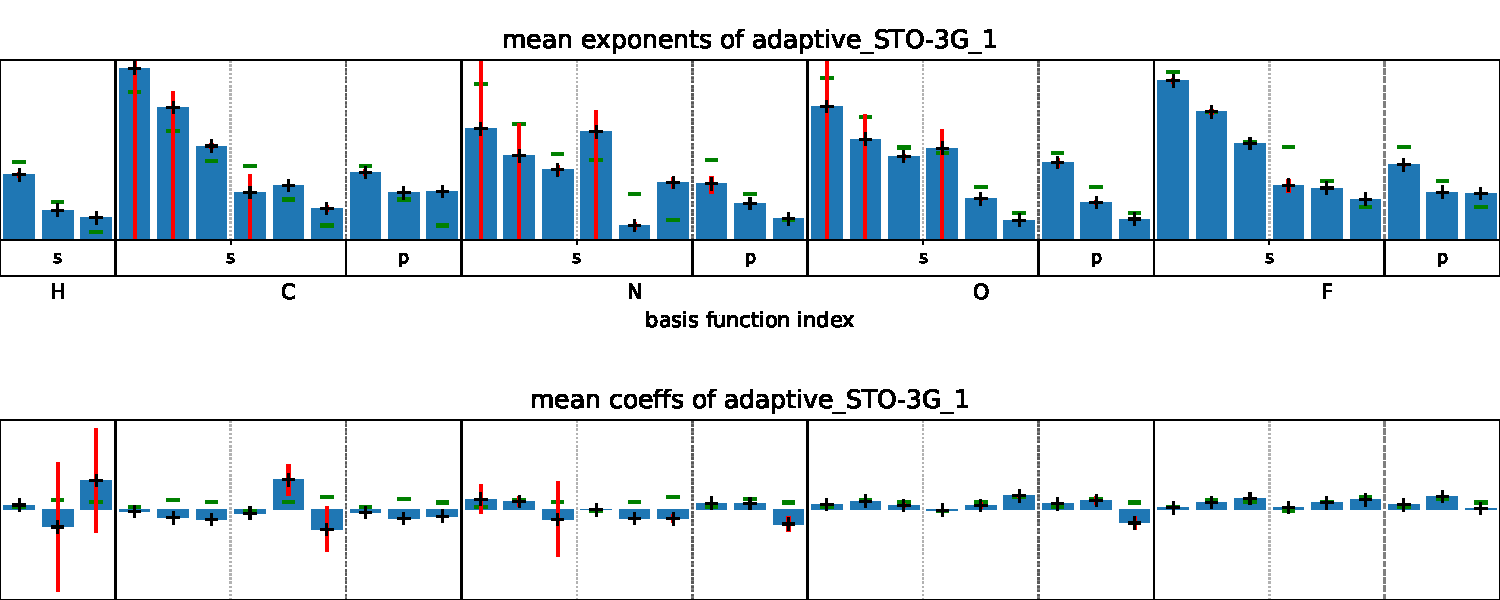
\includegraphics[width=0.75\textwidth]{chapters/results/results_images/adaptive_basis_functions/mean_exps_and_coeffsadaptive_STO-3G_1}
    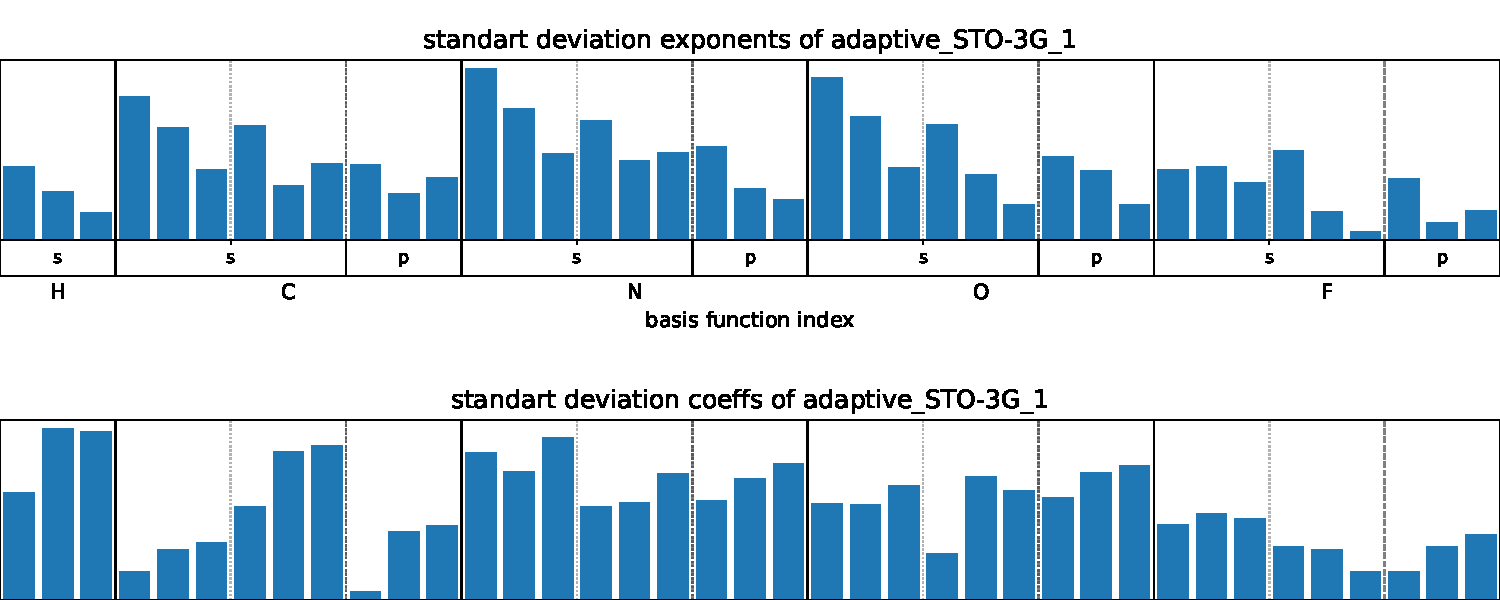
\includegraphics[width=0.75\textwidth]{chapters/results/results_images/adaptive_basis_functions/std_exps_and_coeffsadaptive_STO-3G_1}
    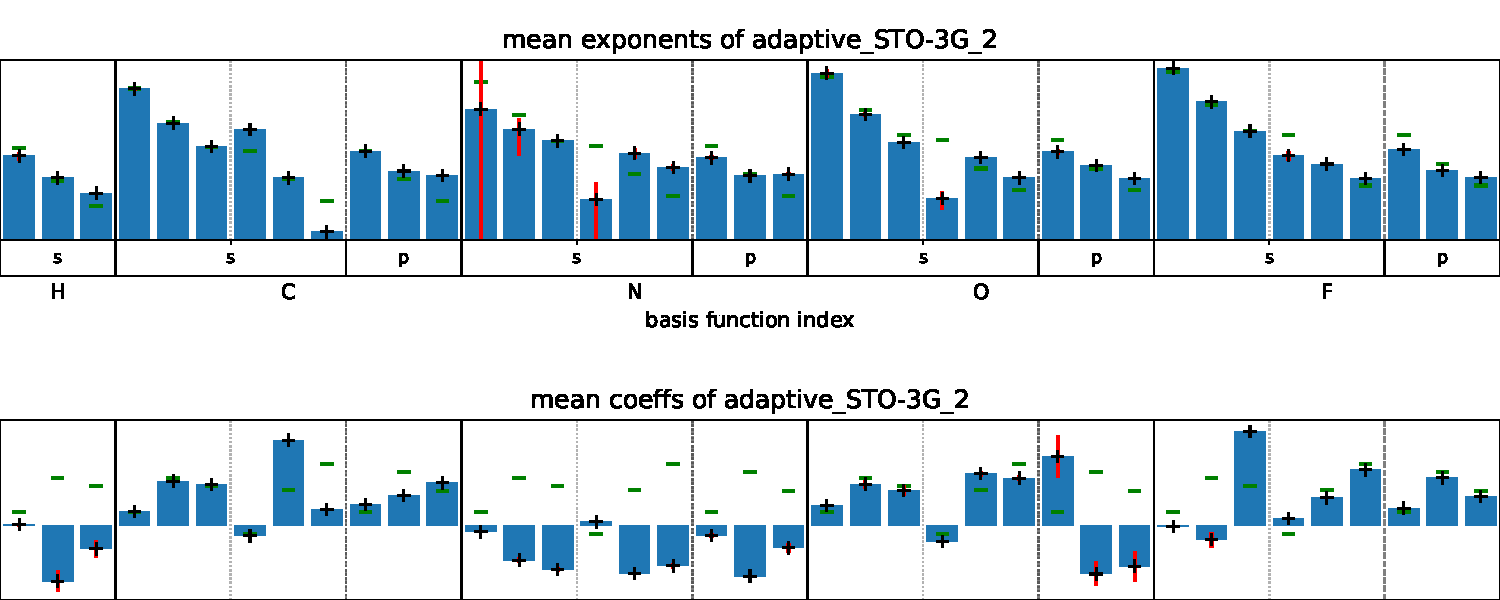
\includegraphics[width=0.75\textwidth]{chapters/results/results_images/adaptive_basis_functions/mean_exps_and_coeffsadaptive_STO-3G_2}
    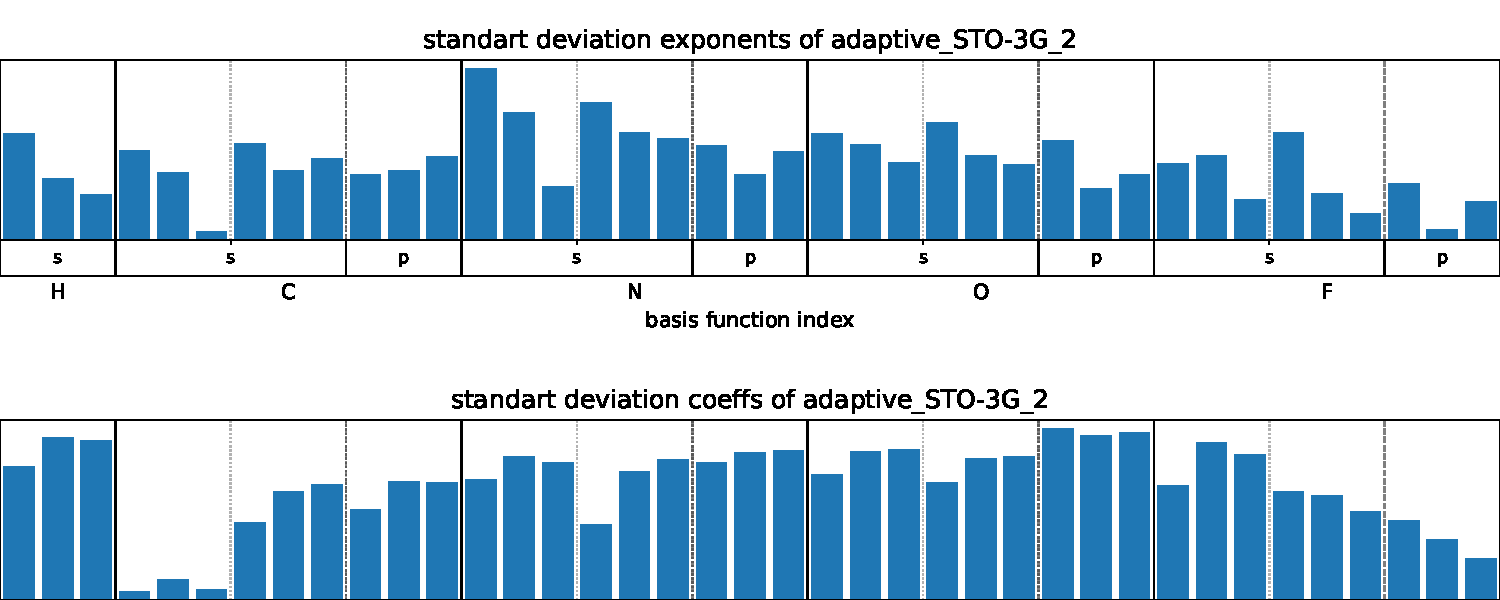
\includegraphics[width=0.75\textwidth]{chapters/results/results_images/adaptive_basis_functions/std_exps_and_coeffsadaptive_STO-3G_2}
    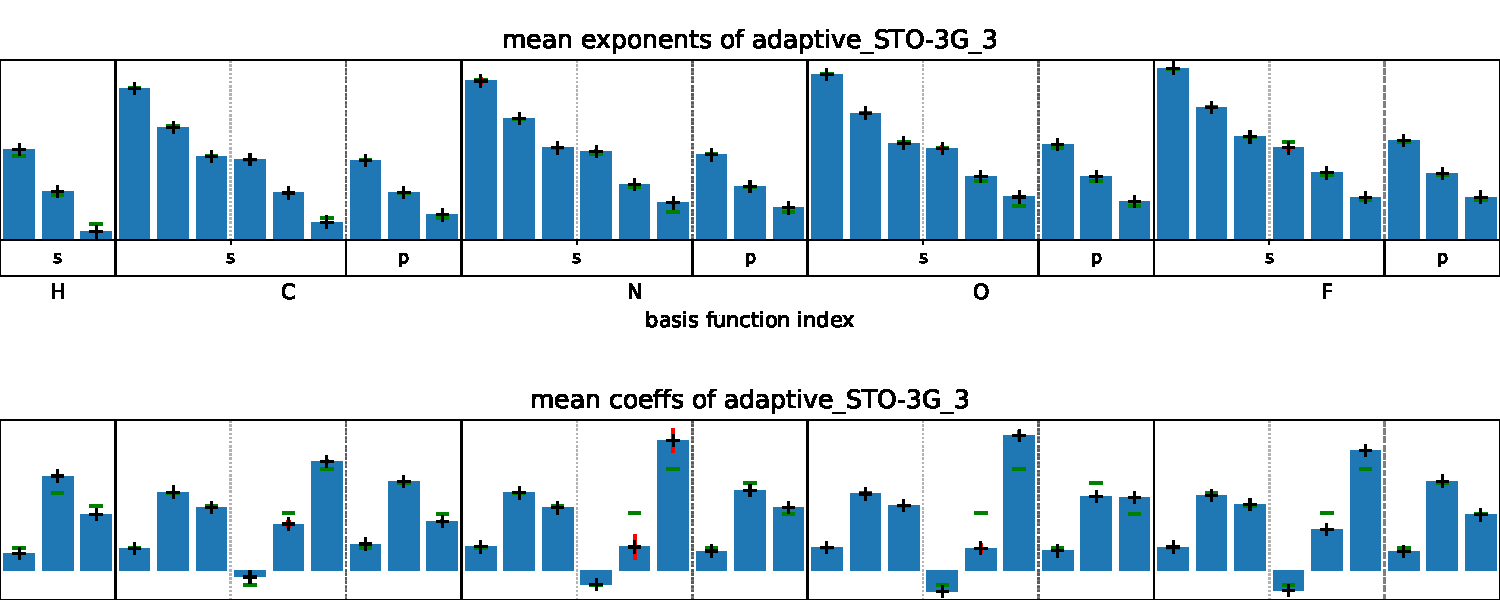
\includegraphics[width=0.75\textwidth]{chapters/results/results_images/adaptive_basis_functions/mean_exps_and_coeffsadaptive_STO-3G_3}
    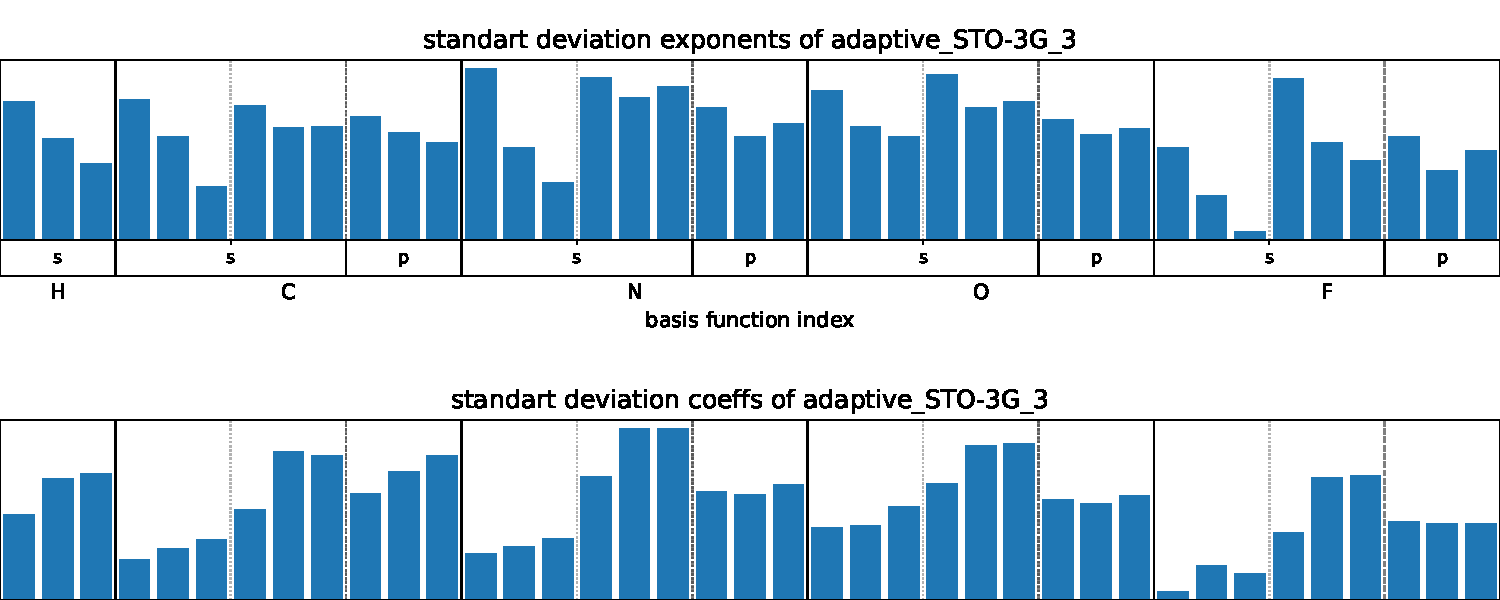
\includegraphics[width=0.75\textwidth]{chapters/results/results_images/adaptive_basis_functions/std_exps_and_coeffsadaptive_STO-3G_3}
\end{figure}


